\documentclass[10pt,twocolumn,letterpaper]{article}

\usepackage{cvpr}
\usepackage{times}
\usepackage{epsfig}
\usepackage{graphicx}
\usepackage{amsmath}
\usepackage{amssymb}
\usepackage{float}

\usepackage{caption}
\usepackage{subcaption}

% Include other packages here, before hyperref.
\setlength{\intextsep}{8pt plus 2pt minus 2pt}

% If you comment hyperref and then uncomment it, you should delete
% egpaper.aux before re-running latex.  (Or just hit 'q' on the first latex
% run, let it finish, and you should be clear).
\usepackage[breaklinks=true,bookmarks=false]{hyperref}

\cvprfinalcopy % *** Uncomment this line for the final submission

\def\cvprPaperID{****} % *** Enter the CVPR Paper ID here
\def\httilde{\mbox{\tt\raisebox{-.5ex}{\symbol{126}}}}

% Pages are numbered in submission mode, and unnumbered in camera-ready
%\ifcvprfinal\pagestyle{empty}\fi
\setcounter{page}{1}
\begin{document}
\vspace{-0.5cm}

%%%%%%%%% TITLE

\title{EE3 Deep Learning Final Report}
\vspace{-0.5cm}

\author{Alexander Montgomerie-Corcoran\\
{\tt\small CID: 01052454, am9215@ic.ac.uk}
}

\maketitle
%\vspace{-0.3cm}
%\thispagestyle{empty}


%%%%%%%%% ABSTRACT
\begin{abstract}
%\vspace{-0.5cm}
   This work investigates descriptor learning for the N-HPatches dataset, a noisy version of the HPatches dataset \cite{hpatches_2017_cvpr}. The descriptors generated are evaluated using the HPatches benchmark\footnote{https://github.com/hpatches/hpatches-benchmark}.
   A baseline approach is taken by first performing denoising using an auto-encoder architecture, and descriptor learning using a convolutional neural network feature extractor. The baseline method achieves \textbf{0.232 mAP} for matching, \textbf{0.541 mAP} for retrieval and \textbf{0.827 mAP} for verification.
   
   The improved approach addresses noise-types applied to the dataset directly as well as exploring different loss functions, achieving \textbf{0.274 mAP} for matching, \textbf{0.560 mAP} for retrieval and \textbf{0.851 mAP} for verification.
\end{abstract}

%TODO: add i
%\vspace{-0.7cm}

%%%%%%%%% BODY TEXT
\section{Introduction}
%\vspace{-0.2cm}

\subsection{Dataset}
%\vspace{-0.2cm}


The HPatches dataset consists of sequences of patches extracted from various images. For every reference image, there is a set of patch sequences for the same subject with either viewpoint changes or illumination changes. These illumination variations can be characterised as varying brightness across the reference image. Viewpoint changes come from different perspectives of the subject, as well as artificial geometric noise applied to the patches. These non-reference sequences are ranked by the magnitude of their viewpoint and illumination variation, and are either \textit{easy, hard} or \textit{tough}. There are 5 patches of each. N-HPatches has an additional random pixel noise applied to each patch.

This dataset consists of 32x32, grayscale images of each patch.
In the training set, there are roughly 1558960 patches from 76 images, and for the test set 952512 patches from 40 images.
The descriptors generated for a patch are 128 scalar features.

%\vspace{-0.2cm}

\subsection{Tasks}
%\vspace{-0.2cm}

The learned descriptors are benchmarked using three different problem classes. 
The patch verification task consists of classifying the similarity of individual patches. This is done by calculating a distance metric between two descriptors of the reference and test patch.
Image matching tasks compare a pair of patch sequences of from images to determine if they are from the same image. 
The patch retrieval task finds a patch corresponding to the reference patch within a pool of patches. 
It is therefore important that descriptors have strong discriminant features of the relevant patch.

%\vspace{-0.2cm}
\section{Baseline Approach}
%\vspace{-0.2cm}


The baseline method approaches the problem by separating denoising and descriptor learning, and employs popular methods for each. 
%The baseline approach takes a uniform approach to each task, and splits up the problem into two sections: patch denoising and patch descriptor.

%\vspace{-0.2cm}
\subsection{Patch Denoising}
%\vspace{-0.2cm}

The patch denoising network makes use of U-Net \cite{RonnebergerFB15}, a popular image segmentation network with use in denoising tasks aswell \cite{unet_example}. This network
acts as an autoencoder, extracting a reduced set of generative features with the encoder path. The features are then decoded, and skip connections are used to propgate any information lost during encoding on the decoder path. 
This network is trained on noisy images evaluated against noiseless images, using Mean Absolute Error (MAE) as the loss function.%, given by Eq. \ref{eq:mae}. 

%\begin{equation}
%    MAE(x,y) = \frac{1}{N} \sum_{i=0}^N | x_i - y_i | 
%    \label{eq:mae}
%\end{equation}

where $x$ and $y$ are the de-noised and clean images respectfully, and $N$ is the folded size of the image (32x32).

The denoise network was trained using an SGD-nesterov optimiser with learning rate 0.00001 and momentum 0.9 over 50 epochs, with a batch size of 500.

%Figure \ref{fig:denoise_loss} shows that it is able to converge to reach both low validation and training loss, however looking at example outputs in Figure \ref{fig:denoise_image}, there is obvious variation between the example and denoised image. Specifically, there is significantly more blurriness compared to the clean network. Although the network appears to have trained well, it has not captured the significant discriminative features of each patch, due the averaging of the loss function.

% could also look at this problem in a different domain.  
%\vspace{-0.2cm}
\subsection{Patch Descriptor}
%\vspace{-0.2cm}

A network is defined to extract discriminant features of each patch. This network is derived from L2-Net \cite{8100132}, a patch descriptor network which employs deep learning techniques.
The network consisted of convolutional layers which extract shift-invariant, discriminant features of the patch. A fully connected layer is used to obtain the most significant features. This network is trained with triplet loss, given by Eq. \ref{eq:triplet_loss}.  

\vspace{-0.2cm}
\begin{equation}
    triplet\_loss(a,n,p) = max(|| a - p ||_2 - || a - n ||_2 + 1,0)
    \label{eq:triplet_loss}
\end{equation}
\vspace{-0.2cm}

where $a$ is the anchor patch output, $p$ is a matching patch output, and $n$ is a non-matching patch output. This loss function gives the network the objective of minimising the L2 distance between matching patches whilst ensuring non-matching are a distance of 1 away.

Stochastic Gradient Descent (SGD) with learning rate of 0.1 is used, and is trained across 50 epochs with a batch size of 50, using 100000 triplets for training and 10000 for validation. The descriptor network was trained using noisy patches processed by the trained denoise network.

%The network learns features such that the L2 distance \cite{DANIELSSON1980227} is maximised between reference and negative features, and minimised between positive and reference features.
% TODO: report timing, all that shit




\subsection{Evaluation}

The baseline method achieves \textbf{0.232 mAP} for matching, \textbf{0.541 mAP} for retrieval and \textbf{0.827 mAP} for verification.
The verification score is similar to that of L2Net for the regular HPatches dataset, however the matching and retreival scores are a lot lower. 


\section{Improved Approach}

To improve on the baseline method, two aspects to the problem are addressed in the improved network. Firstly, the network architecture attempts to directly reduce the impact of all the types of noise applied to the images to reduce the difficulty of learning discriminative features. Secondly, loss functions used in the baseline approach are reviewed in order to find the optimal learning objective for the network. 

\begin{figure}[H]
\centering
  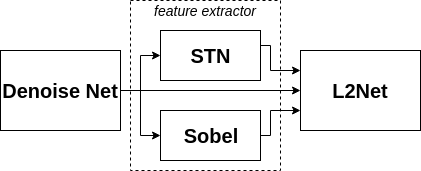
\includegraphics[width=0.77\linewidth]{report/figures/net_overview.png}
  \caption{Overview of full network architecture}
  \label{fig:full_net}
\end{figure}

As seen in Figure \ref{fig:full_net}, the improved architecture follows the baseline method of sequential denoising and descriptor learning stages, with an additional feature extractor stage in between. Although the improvements to each stage are evaluated independently, The overall training is performed on the entire network.

%To improve on the de-noising network, loss functions such as L1 loss and SISSM will be investigated, as they have proven more appropriate for image reconstruction tasks \cite{something}. 

%TODO: network map

%To improve on the de-noising network, loss functions more appropriate for image-based tasks such as SSIM \cite{ZhaoGFK15}will be investigated. As the denoise network uses an averaging loss, there is inherent blurriness at the output such as in Fig. \ref{fig:denoise_image}. Further improvements can be made by assuming additive noise, reducing the compexity of the networks.

%An initial improvement can be made to the descriptor network by identifying existing networks \cite{Tian_2017_CVPR}\cite{Serra_2015_ICCV}\cite{BalntasJTM16}\cite{BMVC2016_119} with better performance, such as HardNet \cite{MishchukMRM17}.
%It would be interesting to investigate domain transforms on the data, such as 2D FFT \cite{rippel2015spectral}, and how this could improve on discriminative ability of the network. A general goal is to address geometric noise more directly.
%It would interesting to expand on this by transforming the domain of the data, appling kernel methods within the network, in particular, how kernels such as the radial basis function can improve discriminative features of the descriptors.

\subsection{Improved Denoise Network}
In the baseline approach, an autoencoder approach is taken towards the problem of denoising images. This technique reduces the discriminative properties of the overall network, as the encoder path learns generative features. The method taken is this work attempts to learn the noise patterns instead, finding features which are orthogonal to that of the original image.

\begin{figure}[H]
\centering
  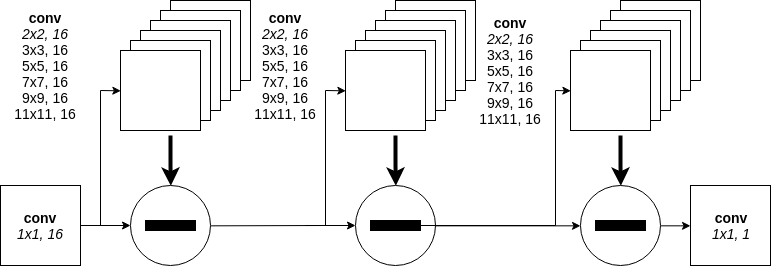
\includegraphics[width=0.99\linewidth]{report/figures/denoise_net_horizontal.png}
  \caption{Denoising network architecture.}
  \label{fig:denoise_net}
\end{figure}

Figure \ref{fig:denoise_net} outlines the overall denoise architecture. The fundamental purpose of this architecture is to remove Additive Gaussian Noise from the image, as this is the noise assumed to be applied to the dataset. There are existing architectures addressing the same problem \cite{ZhangZCM016}, which take a similar approach to learning noise features specifically. 

If it is assumed that the input image, $I_{in}$ is transformed such that $I_{out} = I_{in} + n$, then $I_{in}$ can be recovered such that $\Tilde{I_{in}} = I_{out} - g(I_{out})$. In this network, convolution layers are used such that for a layer with filters $f$, $g(I) = I * f$. Therefore, $f$ is chosen such that $I_{in} * f = 0$ and $\Tilde{I_{in}} = I_{out} - I_{out}*f = I_{out} - I_{in}*f - n*f$.

The network uses a set of convolution layers for noise elimination, with kernel sizes 2,3,5,7,9,11, and depth 16. The many different kernel sizes and relatively small set of filters is to capture the varying frequency of noise.
Sequential noise elimination stages were chosen, such that each subsequent stage can address any residual noise from the previous. 
The number of stages were chosen through evaluation.
%Only three stages were used to avoid over-fitting.

%TODO:
% - mention additive noise
% - learning what's orthogonal to features

Another factor explored with the denoise network is different loss functions. The baseline loss function, MAE, can potentially lead to more blurry images due to the averaging used. This report evaluates two different loss functions: Structural Similarity Index (SSIM) loss and peak signal-to-noise ratio (PSNR) loss, shown in Eq. \ref{eq:denoise_loss},

\begin{equation}
\begin{split}
     ssim\_loss(I_1,I_2) = 1 - \frac{ (2\mu_1 \mu_2 + k_1^2)(2\sigma_{12} + k_2^2) }{ (\mu_1^2 + \mu_2^2 + k_1^2)(\sigma_1^2 + \sigma_2^2 + k_2^2) } 
     \\
 psnr\_loss(I_1,I_2) = - 10 \log_{10} \left( \frac{ M \cdot N }{ \sum_{M,N} ( I_1 (m,n) - I_2 (m,n) )^2 } \right)
\end{split}
\label{eq:denoise_loss} 
\end{equation}

where $I_1,I_2$ are the clean and denoised images, $\mu_1,\mu_2$ are their respective pixel average, $\sigma_1,\sigma_2$ are the respective pixel variance, $\sigma_{12}$ is the covariance, $k_1, k_2$ are constants and $M,N$ are the dimensions of the image.

%TODO: explain variables

%TODO: write loss functions

PSNR is a common image quality indicator, which gives a large penalty to pixels with a big difference to the original, however it has been remarked that this index does not necessarily portray if an image is subjectively similar \cite{6467150}. SSIM uses luminescence, contrast and structure properties to compare images. This index has shown to give good performance in a denoising context \cite{7797130}.

\subsection{Improved Descriptor Network}

To address both geometric noise and illumination variance across patches, two additional components are introduced into the network: a Spatial Transform Network (STN) layer and a Sobel filter. 

The STN layer \cite{jaderberg2015spatial} attempts to learn affine transforms which reduce the geometric noise between a patch sample patch and it's reference. Geometric noise creates difficulties for traditional CNN networks, as they are able to learn translation-invariant features however struggle to learn affine-transform-invariant features. Within standard neural network architectures, only max-pooling layers show any spatial invariance \cite{4270182}. The STN layer addresses this by learning features such as patch orientation and so on to create coefficients which are able to align the geometrically-distorted patches to their original view. 

\begin{equation}
    STN(x_i,y_i)
    = \begin{bmatrix}
    \theta_{11}  & \theta_{12} & \theta_{13} \\
    \theta_{21}  & \theta_{22} & \theta_{23} 
\end{bmatrix}
\begin{bmatrix}
    x_i \\
    y_i \\
    1
\end{bmatrix}
\label{eq:affine_transform}
\end{equation}

The affine transform is given by Eq. \ref{eq:affine_transform}, where $x_i,y_i$ are the co-ordinates of pixel $i$, and $\theta_n$ are the coefficients of the affine transform. The STN layer uses a localisation network to learn the coefficients for the affine transform. 



\begin{figure}[H]
\centering
  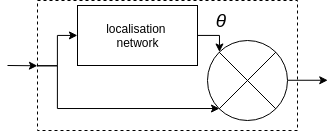
\includegraphics[width=0.7\linewidth]{report/figures/stn_network.png}
  \caption{STN Layer diagram.}
  \label{fig:stn_diagram}
\end{figure}

The localisation network used in this work follows the network presented in \cite{jaderberg2015spatial}. 
The localisation network was initially evaluated using reference and geometrically distorted patches, with MAE loss applied to the processed distorted patch and reference.
It was found that there was not much space for optimisation of the localisation layer, as the network converged very quickly with agreeable results (see Figure \ref{fig:stn_output}).

%It is worth noting that it may seem contradictory to use a CNN to learn affine transforms where previously  

The other type of noise introduced into the network is illumination noise. To address this, illumination invariant features are needed. The approach taken in this work is to use a Sobel filter \cite{sobel_filter} in order to remove any illumination across the image and only give structural features of the patch.  The Sobel filter has been investigated in the context of illumination invariance by Arandiga \textit{et al.} \cite{Arandiga2010}, and has shown good baseline performance in this task with little cost. Especially since these patches cover such a small area of the overall image, there is very little local illumination variance, making the problem a lot simpler. 

\begin{figure}[H]
\centering
  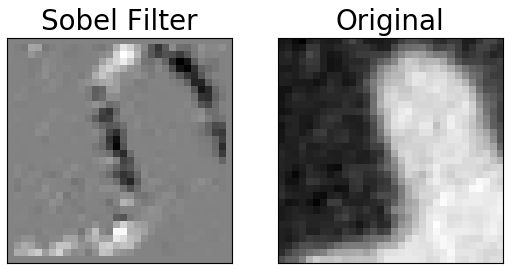
\includegraphics[width=0.55\linewidth]{report/figures/sobel_filter.png}
  \caption{Sobel Filter output.}
  \label{fig:sobel_filter_output}
\end{figure}

From Figure \ref{fig:sobel_filter_output}, it can be seen that only edges within the patch are observed at the output, thus removing features caused by uniform illumination across the patch.


%\begin{figure}[H]
%\centering
%  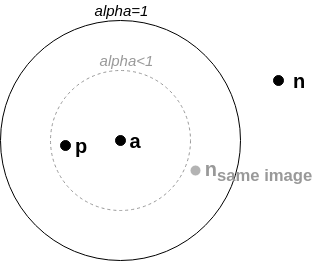
\includegraphics[width=0.50\linewidth]{report/figures/triplet_loss.png}
%  \caption{Triplet Loss with regularisation for patches of the same image.}
%  \label{fig:triplet_loss}
%\end{figure}

Finally, the last improvement investigated is with regards to the overall loss function. Intuitively, a good patch descriptor must not only hold patch-specific information, but also have some features which are common to patches of the same image. Specifically for the image matching task, patches of the same image should show some similarity despite being different patches. This principal is implemented as a form of regularisation to the original triplet loss.

\vspace{-0.5cm}
\begin{equation}
    triplet\_loss\_r(a,p,n) = max(|| a - p ||_2 - || a - n ||_2 + \alpha,0) 
\end{equation}
\vspace{-0.2cm}

where $\alpha=1$ if they are not the same patch, $\alpha=0$ if they are the same patch, and $\alpha<1$ if they are different patches but of the same image. 
%The loss function is illustrated in Figure \ref{fig:triplet_loss}. 
This regularisation hopes to improve generalisation of the descriptor, however can have impact on intra patch verification tasks, which the hyperparameter $\alpha$ governs.

 
\subsection{Evaluation}
\label{sec:evaluation}

\subsubsection{Denoise Network}

For choosing the number of layers for the improved denoising network, different numbers of layers were evaluated against MAE loss between denoised and clean patches. Each network was trained for 25 epochs using SGD.

\begin{table}[H]
\centering
\begin{tabular}{|l|l|}
\hline
\textbf{Layers} & \textbf{MAE}  \\ \hline
1             & 7.1083   \\ 
2             & 6.2294   \\ 
2             & \textbf{6.0029}   \\ 
4             & 6.0797   \\ \hline
\end{tabular}
\caption{Evaluation of number of layers for the denoising network.}
\label{tab:denoise_loss}
\end{table}

The loss functions were evaluated also. Each network was trained using each loss for 50 epochs and evaluated using the benchmark with the same trained L2Net for each. The results can be seen in Table \ref{tab:denoise_loss}. It is clear that SSIM loss provides the highest precision out of all networks.


\begin{table}[H]
\begin{tabular}{|l|l|l|l|}
\hline
\textbf{Loss} & \textbf{Verification} & \textbf{Matching} & \textbf{Retrieval} \\ \hline
mae                    & 0.745 mAP                   & 0.157 mAP               & 0.465 mAP                \\ 
ssim\_loss             & \textbf{0.773} mAP          & \textbf{0.162} mAP      & \textbf{0.469} mAP       \\ 
psnr\_loss             & 0.752 mAP                   & 0.156 mAP               & 0.466 mAP                \\ \hline
\end{tabular}
\caption{Evaluation of Loss functions for the denoising.}
\label{tab:denoise_loss}
\end{table}
 
\subsubsection{Descriptor Network}

To evaluate which $\alpha$ to use for regularised patches of the same image, different values were evaluated, and shown in Table \ref{tab:alpha_eval}. A network was trained with each $\alpha$ using the improved network for 25 epochs, and evaluated using the benchmark. 50000 training and 5000 test triplets were used at a batch size of 50, using an SGD optimiser.

From the table, it is difficult to determine exactly which value of $\alpha$ to use, as there is no clear trend in results for $\alpha$. It is decided that an $\alpha$ of 0.75 will be used for the final approach, as it shows improvements in matching with little loss in verification score.

\begin{table}[H]
\centering
\begin{tabular}{|l|l|l|l|}
\hline
$\mathbf{\alpha}$ & \textbf{Verification} & \textbf{Matching} & \textbf{Retrieval} \\ \hline
1.0  & 0.822 mAP & 0.217 mAP & 0.507 mAP \\ 
0.75 & 0.819 mAP & 0.222 mAP & 0.507 mAP \\ 
0.5  & 0.814 mAP & 0.213 mAP & 0.503 mAP \\ 
0.25 & 0.821 mAP & 0.215 mAP & 0.506 mAP \\ 
\hline
\end{tabular}
\caption{Evaluation of Loss functions for the denoising.}
\label{tab:alpha_eval}
\end{table}


%\begin{table}[H]
%\begin{tabular}{|l|l|l|l|}
%\hline
%\textbf{Regularised} & \textbf{Verification} & \textbf{Matching} & \textbf{Retrieval} \\ \hline
%False & 0.847 mAP & 0.264 mAP & 0.558 mAP \\ 
%True  & 0.851 mAP & 0.274 mAP & 0.560 mAP \\ 
%\hline
%\end{tabular}
%\caption{Evaluation of Loss functions for the denoising network.}
%\label{tab:denoise_loss}
%\end{table}
 
With regards to the STN layer, it can qualitatively be seen from Fig. \ref{fig:stn_output} that the orientation and scaling of the image is resolved to be the same as the original image. The main difference introduced is the artefacts from the affine transform seen at the edges.
 
\begin{figure}[H]
\centering
  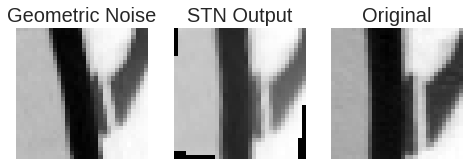
\includegraphics[width=0.85\linewidth]{report/figures/stn_out.png}
  \caption{Example of STN Output.}
  \label{fig:stn_output}
\end{figure}

 
\subsubsection{Improved Network}

The final network was trained in it's entirety, with no weight re-use from individual training of sections. Stochastic Gradient Descent (SGD) with learning rate of 0.1 was used as the optimiser, and the model was trained across 100 epochs, with only the weights leading to the lowest validation loss kept. It was found that using pretrained weights for the denoise network resulted in lower benchmark scores (0.773 mAP, 0.170 mAP and 0.468 mAP for verification, matching and retrieval respectively). Also, for Fig. \ref{fig:triplet_loss_weight_init}, it can be seen that weight initialisation has lead to great variance in validation loss, suggesting the model has overfitted to the training data.

On the contrary, having no weight initialisation leads to smooth training curves and overall higher score. It is hypothesised that by training the whole network from scratch, the denoise network is able to filter out not only pixel-noise but also non-discriminative features.

\begin{figure}[H]
     \centering
     \begin{subfigure}[b]{0.35\textwidth}
         \centering
         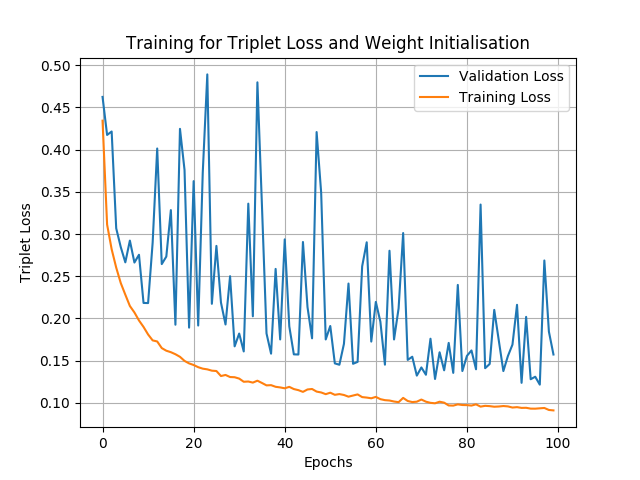
\includegraphics[width=\textwidth]{report/figures/loss_0.png}
         \caption{Triplet Loss, Weight Initialisation}
         \label{fig:triplet_loss_weight_init}
     \end{subfigure}
     %\begin{subfigure}[b]{0.4\textwidth}
     %    \centering
     %    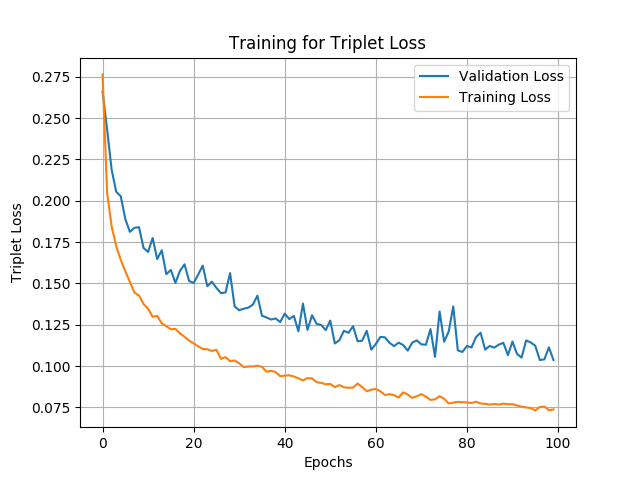
\includegraphics[width=\textwidth]{report/figures/loss_1.png}
     %    \caption{Triplet Loss}
     %    \label{fig:triplet_loss}
     %\end{subfigure}
     \begin{subfigure}[b]{0.35\textwidth}
         \centering
         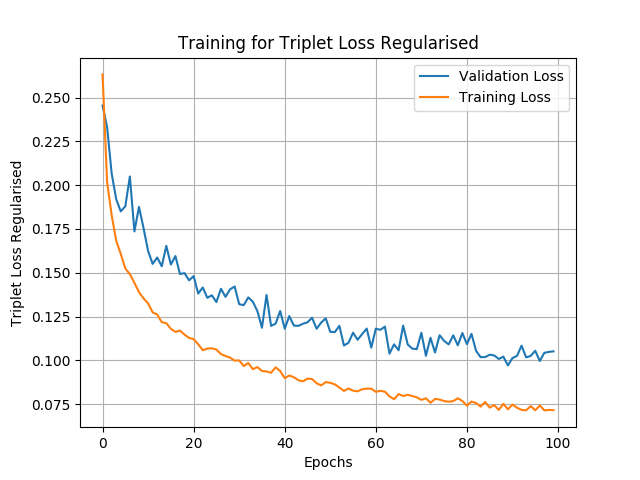
\includegraphics[width=\textwidth]{report/figures/loss_2.png}
         \caption{Triplet Loss with Regularisation, no Weight Initialisation}
         \label{fig:triplet_loss_regularised}
     \end{subfigure}
        \caption{Training and validation loss for different configurations of the improved network.}
        \label{fig:training_val_loss_improved}
\end{figure}

The network was able to achieve \textbf{0.851} mAP, \textbf{0.274} mAP and \textbf{0.560} mAP scores for Verification, Matching and Retrieval tasks respectively. The full network was also evaluated without regularisation, however received 0.004 mAP, 0.01 mAP, and 0.002 mAP less in Verification, Matching and Retrieval tasks respectively. 
%These results are comparable to the results of L2-Net for the original HPatches dataset, suggesting the network is able to handle the image noise effectively. This has an incremental improvement on the baseline method.
The greatest improvement from the baseline is in the image matching benchmark, suggesting the new loss function contributes is effective in it's goal.


%TODO: describe training procedure
 
{\small
\bibliographystyle{ieee}
\bibliography{egbib}
}

\appendix

\section{Baseline Training}
The training curves for the baseline Denoise network are given in Fig. \ref{eq:denoise_loss}, and the L2Net training curve is given in Fig. \ref{fig:descriptor_loss}.

\begin{figure}[H]
\centering
  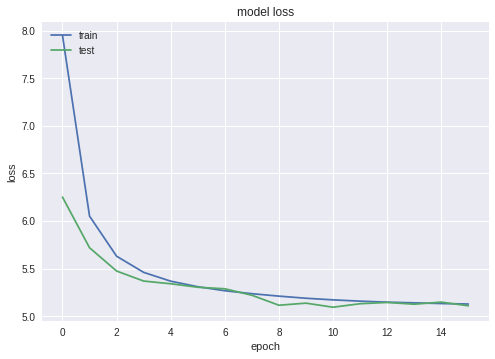
\includegraphics[width=0.65\linewidth]{figures/denoise_train.png}
  \caption{Baseline Denoising Network Loss against Epochs.}
  \label{fig:denoise_loss}
\end{figure}


\begin{figure}[H]
\centering
  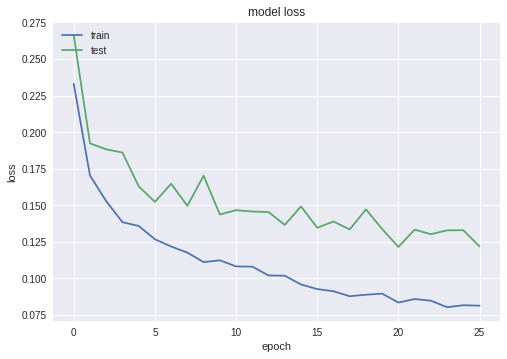
\includegraphics[width=0.65\linewidth]{figures/descriptor_train.png}
  \caption{Baseline Descriptor Network Loss against Epochs.}
  \label{fig:descriptor_loss}
\end{figure}

\section{Improved Denoise Network Notes}

The output of the improved denoise network with SSIM loss, seen if Fig. \ref{fig:denoise_image}, is able to perform denoising fairly well. 

\begin{figure}[H]
\centering
  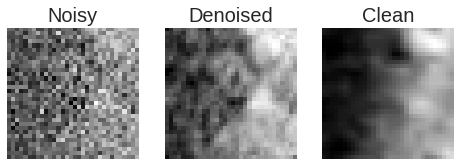
\includegraphics[width=0.65\linewidth]{report/figures/denoise_image.png}
  \caption{Improved Denoising Network Output Example.}
  \label{fig:denoise_image}
\end{figure}

Qualitively, it can also be seen that the features learned in the training network are not typical smooth feauture learned, and from Figure \ref{fig:denoise_weights} the weights of the first layer for kernel size of 11 appear to be very noisy and void of the common shapes found in weights of CNNs.

\begin{figure}[H]
\centering
  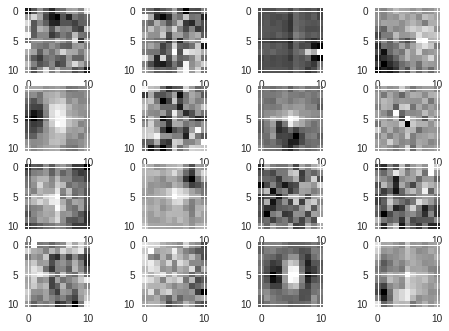
\includegraphics[width=0.7\linewidth]{report/figures/denoise_weights.png}
  \caption{Visualisation of Denoise Network Weights.}
  \label{fig:denoise_weights}
\end{figure}

\section{Pledge}
\textit{I, Alexander Montgomerie-Corcoran, pledge that this assignment is completely my own work, and that I did not take,
borrow or steal work from any other person, and that I did not allow any other person to use, have, borrow
or steal portions of my work. I understand that if I violate this honesty pledge, I am subject to disciplinary
action pursuant to the appropriate sections of Imperial College London.}
\\
\\
I have discussed my work with Martin Ferianc.


\end{document}
